\section{Related Work}
\label{sec:related_work}

%% Long version below if you need more context!
\textbf{System Identification.}
Physical parameters such as stiffness or relaxation behavior are rarely known precisely for real-world scenes, which limits the use of \gls{pde} simulators in many engineering applications~\citep{landau2012theory, blazek2015computational, salatovic2025reliable, avril2017material, chai2024smart}.
System identification~\citep{aastrom1971system, lennart1999system} recovers such parameters from indirect observations.
In applied mechanics, related approaches include finite element model updating and the Virtual Fields Method~\citep{avril2008overview, pierron2010extension, bonnet2005inverse}.
Recent approaches pair learned models with physics engines or differentiable simulators for property estimation and control~\citep{wu2015galileo, murthy2020gradsim, antonova2023rethinking}, and train surrogate models for \gls{pde}-constrained parameter inference~\citep{qzhao2022graphpde, wang2024latent, adaptigraph24}.
% Simulators are critical for solving \glspl{pde} across a number engineering applications, yet essential physical parameters such as stiffness or relaxation behavior are rarely known precisely for a given real-world scene~\citep{landau2012theory, blazek2015computational, salatovic2025reliable, avril2017material, chai2024smart}.
% System identification \citep{aastrom1971system, lennart1999system} addresses this by recovering parameters from indirect observations, with counterparts in applied mechanics spanning updating of finite element models to the Virtual Fields Method \citep{avril2008overview, pierron2010extension, bonnet2005inverse}.
% and identifiability-aware analyses of nonlinear constitutive laws \citep{zhang2022parameter}.
% Learning-based variants couple deep models to physics engines for property estimation from video data \citep{wu2015galileo}, use differentiable simulators for gradient-based identification and control \citep{murthy2020gradsim, antonova2023rethinking}, or invert learned surrogates for \gls{pde}-constrained inverse problems and online property estimation \citep{qzhao2022graphpde, wang2024latent, adaptigraph24}.
% Learning-based approaches combine deep models with physics engines or differentiable simulators for property estimation and control \citep{wu2015galileo, murthy2020gradsim, antonova2023rethinking}, and extend to inverse problems by learning surrogate models for \gls{pde}-constrained parameter inference \citep{qzhao2022graphpde, wang2024latent, adaptigraph24}.

A different line of robotic real-to-sim work recovers deformable-object parameters via a per-instance test-time optimization.
These works include iterative FEM-comparison \citep{frank10}, to differentiable rendering and simulation \citep{diffcloud22}, to differentiable-simulator system identification on point clouds \citep{yang2025differentiable, adaptigraph24}.
Each instance requires a fresh optimization, which is typically done iteratively. 
The objective is non-convex and exhibits local minima and sloppy parameter directions~\citep{transtrum2010nonlinear, zhang2022parameter}. 
Direct-inversion alternatives sidestep the non-convexity but require dense full-field strain measurements~\citep{avril2008overview} that are unavailable in typical real-world settings.
\gls{peach} amortizes identification into a learned encoder, replacing per-instance optimization with a single forward pass, and we compare against a test-time optimization baseline in Section~\ref{sec:experiments}.



% These methods trigger a fresh inference step per instance that requires the forward model to remain well-conditioned: the iterative-optimization majority is additionally non-convex with documented local minima and sloppy parameter directions \citep{transtrum2010nonlinear, zhang2022parameter}, while direct-inversion methods avoid this only by requiring dense full-field strain measurements \citep{avril2008overview} unavailable from typical real-world sensing.
% \gls{peach} amortizes identification into a learned encoder: a single forward pass replaces the inner step, and although our forward simulator is differentiable, we avoid test-time optimization both because it scales poorly across many instances and because the inverse problem is generally ill-conditioned \citep{transtrum2010nonlinear, zhang2022parameter}, trading these failure modes for the more controllable one of imperfect generalization from training data.


\textbf{Adapting Learned Simulators to New Materials.}
% S1 — GNS as the relevant family
Graph network simulators have emerged as fast, differentiable surrogates for mesh- and particle-based physics, enabling scalable simulation of physical systems of rigid bodies \citep{battaglia2016interaction, sanchezgonzalez2020learning}, deformable solids~\citep{pfaff2020learning}, and PDE-like dynamics on unstructured meshes~\citep{brandstetter2021message}. 
Recent extensions aim to capture long-range interactions in nonlinear solid mechanics via hierarchical architectures \citep{yu2024learning, freymuth2025amber, wurth2025diffusion}.
% S2 — Adjacent paradigms
% S3 — The adaptation problem within learned simulators
These methods assume known process conditions and thus inherit the parameter-estimation problem whenever materials change.
Recent work therefore conditions learned simulators on material parameters either via parameter-efficient fine-tuning \citep{manoharan2025parameter} or via meta-learning over a context set of trajectories \citep{chakrabarty2025meta, dahlinger2025context}.
% S4 — In-context conditioning, MaNGO as the closest neighbor

In particular, MaNGO \citep{dahlinger2025mango} encodes a context set of mesh trajectories into a latent material descriptor that conditions a trajectory-level \gls{gns}, enabling adaptation to unseen materials in a single forward pass without test-time optimization. 
This is achieved via a \glsf{cnp} formulation for in-context learning \citep{garnelo_conditional_2018}.
% S5 — The gap, with goal/method distinction
However, mesh trajectories of arbitrarily deforming objects are not directly observable with real-world sensors, limiting MaNGO to synthetic data regimes.
% Since our objective is real-to-sim adaptation across varying material conditions
Instead, we condition on point cloud sequences, enabling adaptive physical simulation of real scenes with readily available 3D cameras.
Recent advances in foundation models for stereo reconstruction further support this approach by enabling the generation of cleaner and less noisy point clouds \citep{wen2025stereo}.

\begin{figure}[!t]
  \centering
  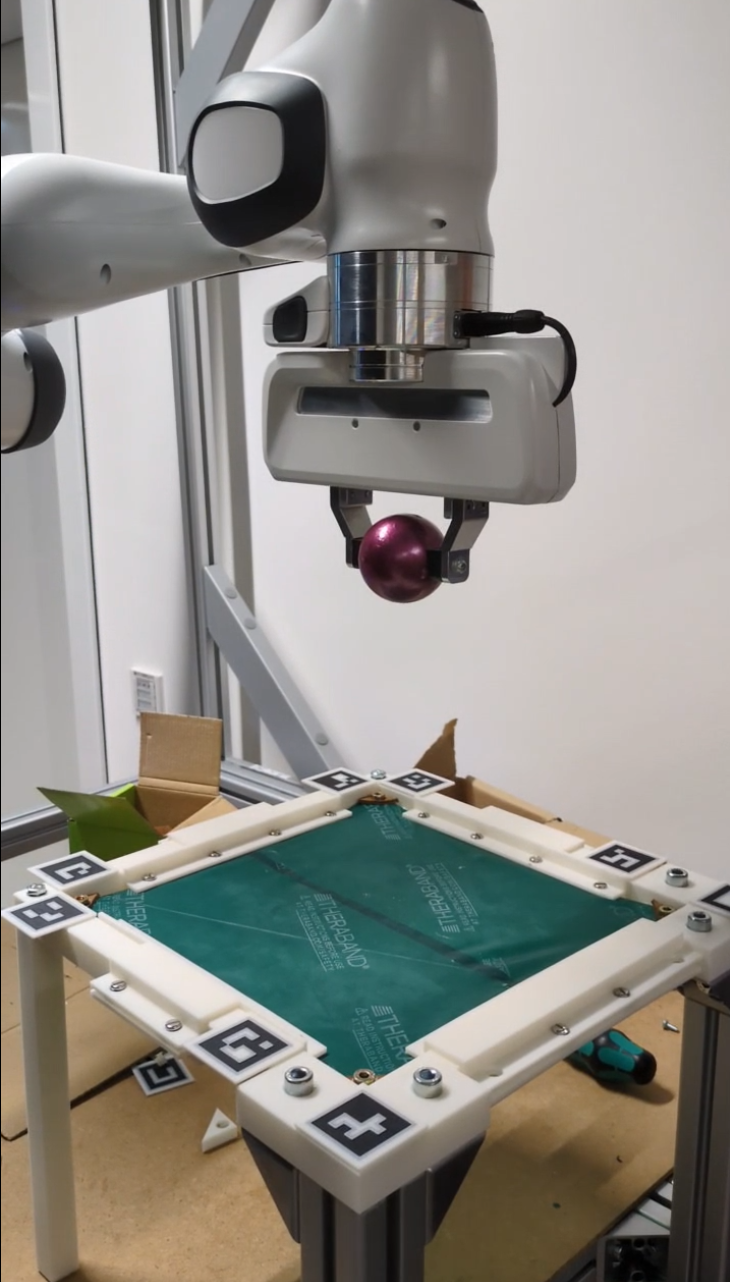
\includegraphics[width=0.192\textwidth, trim={0 2.5cm 0 3.5cm}, clip]{figures/qualitative_realworld_data/01.png}\hfill
  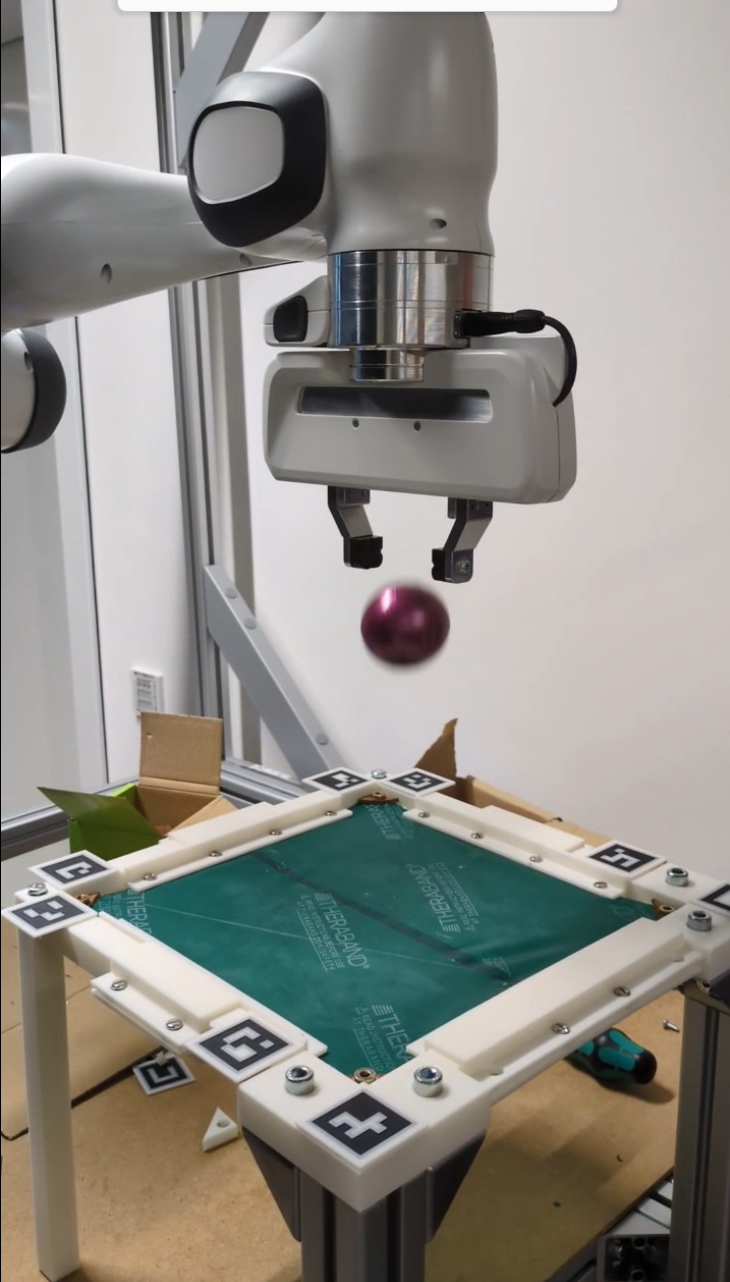
\includegraphics[width=0.192\textwidth, trim={0 2.5cm 0 3.5cm}, clip]{figures/qualitative_realworld_data/02.png}\hfill
  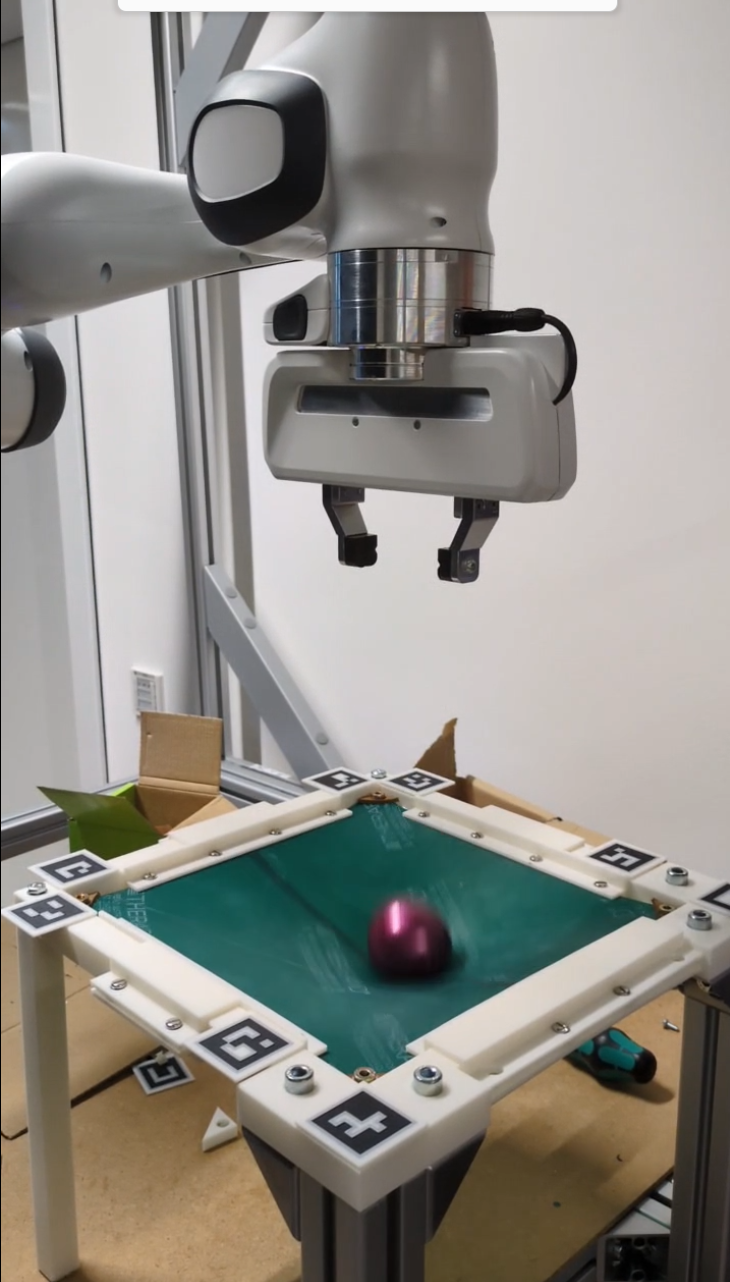
\includegraphics[width=0.192\textwidth, trim={0 2.5cm 0 3.5cm}, clip]{figures/qualitative_realworld_data/03.png}\hfill
  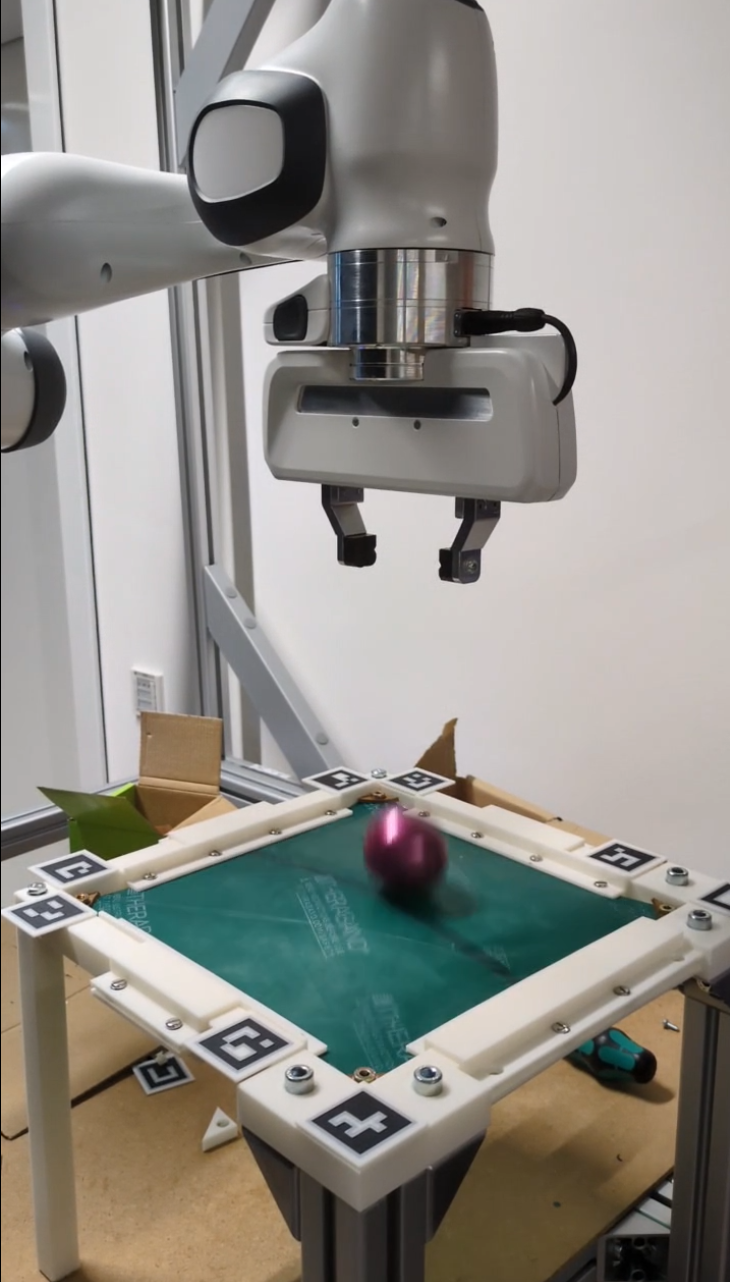
\includegraphics[width=0.192\textwidth, trim={0 2.5cm 0 3.5cm}, clip]{figures/qualitative_realworld_data/04.png}\hfill
  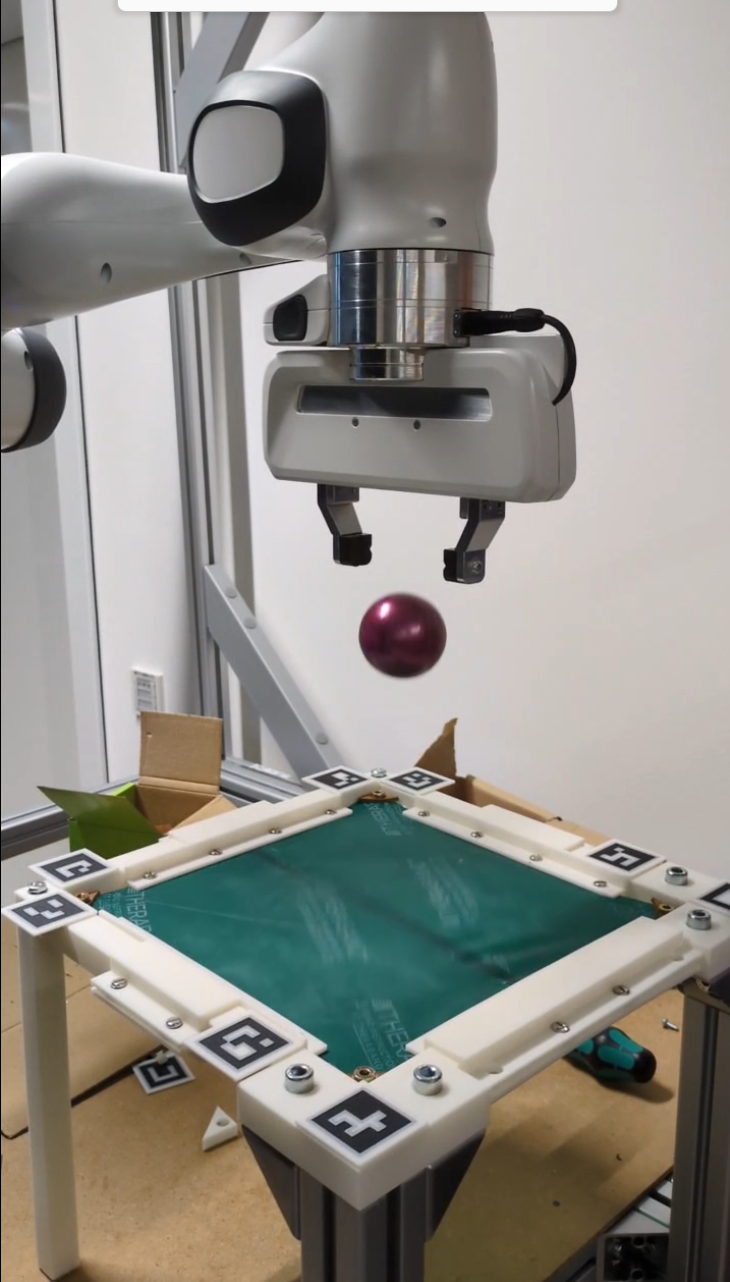
\includegraphics[width=0.192\textwidth, trim={0 2.5cm 0 3.5cm}, clip]{figures/qualitative_realworld_data/05.png}
  \caption{Real-world \texttt{Trampoline} setup. A robot arm releases a steel ball above an elastic membrane stretched across a 3D-printed frame, with ArUco markers at the corners for calibration.}
  \label{fig:realworld_setup}
  \vspace{-0.3cm}
\end{figure}

% Paragraph 3: Positioning, Engine and the Juice
\textbf{Point Cloud Sequence Observations for Learned Simulators.}
While permutation-invariant set encoders for individual point clouds \citep{qi2016pointnet, ruizhongtai2017pointnet, pointMAE, pointBERT, pointGPT} are well-established, processing point cloud sequences requires architectures that handle spatial irregularity and frame-to-frame motion without explicit point correspondences \citep{meteornet19, fan2021pstnet}.
Within learned simulation, point clouds have been used either to ground mesh-based \glspl{gns} in sensor observations~\citep{linkerhagner2023grounding}, or as the basis of particle-based dynamics models that operate directly in observation space for deformable-object manipulation \citep{li2019learning, robocook23}.
% In both cases, they are used to directly drive the dynamics rather than serve as a context representation for material inference.
In both cases, the latent physical properties are implicitly learned in the dynamics model, making adapting to new conditions less data efficient.
Instant Policy \citep{vosylius2024instantpolicyincontextimitation} instead conditions imitation learning policies on point cloud demonstrations via amortized in-context learning. The method shares PEACH's conditioning paradigm but applies to robot policies rather than material parameters and operates without a downstream physics simulator.
% PEACH targets a regime that none of the above categories addresses jointly: amortized in-context real-to-sim adaptation from point cloud sensor data, combining the sequence-encoder lineage of \citep{meteornet19, fan2021pstnet, Gyenes24} with the in-context conditioning paradigm of \citep{vosylius2024instantpolicyincontextimitation, dahlinger2025mango} to bypass both the test-time optimization of differentiable-simulator real-to-sim methods and the mesh-trajectory requirement of prior in-context simulator adaptation \citep{dahlinger2025mango}.

% PEACH targets a regime not jointly addressed by prior work: amortized in-context sim-to-real adaptation from point cloud observations.
% It combines sequence-based point cloud encoders \citep{meteornet19, fan2021pstnet} with in-context conditioning mechanisms \citep{vosylius2024instantpolicyincontextimitation, dahlinger2025mango}, while avoiding both the test-time optimization required by differentiable-simulator real-to-sim methods and the reliance on mesh-trajectory supervision in prior in-context simulator adaptation \citep{dahlinger2025mango}.

% Graph network simulators have emerged as fast, differentiable surrogates for mesh- and particle-based physics, scaling from particle systems and rigid interactions \citep{battaglia2016interaction, sanchezgonzalez2020learning, hd-vpd} to deformable solids and PDE solving on unstructured meshes \citep{pfaff2020learning, brandstetter2021message}, with hierarchical extensions handling long-range collisions and global structural effects in nonlinear solid mechanics \citep{yu2024learning, wurth2025diffusion} and adaptive-resolution meshing \citep{freymuth2025amber}.

% Adjacent paradigms - neural operators in function space \citep{li2021fourier}, equivariant trajectory-level architectures for 3D dynamics \citep{egno2024}, and recent transformer-based neural operators that unify Lagrangian and Eulerian simulation \citep{alkin2024upt, alkin2025abupt} - share the goal of replacing classical solvers with fast, learned surrogates.

% To keep the latent material descriptor from absorbing geometric shortcuts during end-to-end training, we additionally supervise the encoder with a signed-distance reconstruction loss that gives geometry a dedicated output channel and frees the conditioning latent to specialize on material, drawing on implicit geometric representations \citep{park2019deepsdf, mescheder2019occupancy} as auxiliary supervision rather than as a primary modeling objective.




















% Ye olde version

% * We are latent space, while test-time optimization directly does parameter space 
% \todo{Learning-based forward simulators.}
% General learned simulators: \citep{pfaff2020learning,dahlinger2025mango,li2021fourier,yu2023learning,egno2024,brandstetter2021message}
% \todo{Material estimation.}
% \begin{itemize}
%     \item Adaptigraph \citep{adaptigraph24}
%     \item non-learned approach:A robot equipped with a force sensor physically deforms objects while a camera observes the resulting surface changes, which are compared to a finite element simulation to estimate elasticity parameters. \citep{frank10} 
%     \item DiffCloud tackles the real-to-sim problem for highly deformable objects by inferring physical simulation parameters (mass, stiffness) directly from real point cloud observations captured during robot manipulation. It combines differentiable point cloud rendering with differentiable simulation to propagate gradients end-to-end, enabling parameter estimation via gradient descent in roughly 10 minutes rather than the several hours required by inverse model baselines. Apparently it also has an amortized encoder which uses pointnet and meteornet (double check that).\citep{diffcloud22}
% \end{itemize}

% Our novelty: combine learned simulation and parameter estimation from point clouds into a combined framework. Fast adaptation, no optimization at test time, good results, etc.(right?)

% \todo{Point cloud sequence processing}
% \begin{itemize}
%     \item PSTNet \citep{fan2021pstnet}
%     \item Instant Policy \citep{vosylius2024instantpolicyincontextimitation}
%     \item MeteorNet \citep{meteornet19}
% \end{itemize}
% \todo{Learned Simulators that use Pointclouds directly}
% \begin{itemize}
%     \item GGNS \citep{linkerhagner2023grounding}
%     \item RoboCook \citep{robocook23}
% \end{itemize}


% \claude{
% \paragraph{Learning-based forward simulators.}
% A large body of work has demonstrated that graph neural networks (GNNs) are well suited for learning forward simulation of physical systems. MeshGraphNets \citep{pfaff2020learning} introduced mesh-based graph network simulators (GNS) that learn to predict dynamics of deformable solids and fluids directly on unstructured meshes, at a fraction of the cost of classical FEM solvers. MaNGO \citep{dahlinger2025mango} extended this paradigm to the multi-task setting by meta-learning a GNS that rapidly adapts to unseen material configurations. Beyond mesh-based approaches, neural operators such as the Fourier Neural Operator \citep{li2021fourier} and message-passing PDE solvers \citep{brandstetter2021message} learn mappings in function space and generalize across discretizations. Recent work has also explored equivariant architectures for 3D dynamics \citep{egno2024} and hierarchical contact representations for flexible body collisions \citep{yu2023learning}. Our work builds on the mesh-based GNS paradigm but extends it with the ability to infer latent material parameters from observed point cloud sequences, without requiring test-time gradient-based optimization.
% \paragraph{Material parameter estimation.}
% Identifying the physical parameters of deformable objects from observations is a long-standing problem. Early work by \citet{frank10} employed a robot with a force sensor to physically probe objects while comparing observed surface deformations to a FEM simulator, iteratively minimizing the discrepancy to recover elasticity parameters. While effective, this approach requires a differentiable or queryable simulator at test time and is not amortized. DiffCloud \citep{diffcloud22} tackles the same real-to-sim problem by constructing an end-to-end differentiable pipeline that propagates gradients from real point clouds through differentiable rendering and differentiable simulation, enabling parameter estimation via gradient descent in roughly ten minutes. AdaptiGraph \citep{adaptigraph24} learns a physical property-conditioned graph-based neural dynamics model and, upon encountering a new material at deployment time, recovers its properties via online gradient-based optimization over a few observed interactions. In contrast to all of the above, our approach amortizes inference: a learned encoder maps a short sequence of point cloud observations to a latent material representation in a single forward pass, requiring no optimization at test time.
% \paragraph{Point cloud sequence processing.}
% Processing sequences of point clouds is inherently challenging due to the lack of spatial regularity and the need to capture both spatial structure and temporal motion. MeteorNet \citep{meteornet19} proposed direct spatio-temporal convolutions on dynamic 3D point cloud sequences by aggregating local neighborhoods across both space and time. PSTNet \citep{fan2021pstnet} followed a similar philosophy with point spatio-temporal convolutions that decouple spatial and temporal modeling. More recently, Instant Policy \citep{vosylius2024instantpolicyincontextimitation} demonstrated that point cloud sequences can serve as in-context demonstrations for imitation learning, encoding manipulation tasks directly from a handful of observations. Our encoder draws inspiration from this line of work, processing multi-timestep point clouds to extract a compact latent code that characterizes the material properties of the observed object.
% \paragraph{Learned simulators operating on point clouds.}
% A closely related thread of work combines learned simulation with raw sensor observations. GGNS \citep{linkerhagner2023grounding} grounds mesh-based GNSs with real-world point cloud measurements, fusing sensor information into the simulation state at each step to correct for accumulated prediction error and to enable stable long-term rollouts. RoboCook \citep{robocook23} operates on particle-based representations derived from point clouds to model the elasto-plastic dynamics of cooking materials, learning a dynamics model that operates directly in observation space for downstream manipulation planning. Both works demonstrate the value of tightly coupling point cloud observations with learned simulators. Our approach differs in that point clouds serve not as a state correction signal during rollout, but as context from which material parameters are inferred once, enabling a standard mesh-based forward simulator to generalize to new materials at inference time.}